\documentclass{article}

\usepackage{graphicx}
\usepackage{tikz}
\usepackage{tikzsymbols}
\usetikzlibrary{calc,patterns,shapes.geometric}
\pagestyle{empty}
\usepackage[margin=0pt]{geometry}
\geometry{papersize={14in,12in}}

\def\centerarc[#1](#2)(#3:#4:#5){\draw[#1] ($(#2)+({#5*cos(#3)},{#5*sin(#3)})$) arc (#3:#4:#5);}

\begin{document}
	\begin{figure}
		\centering
		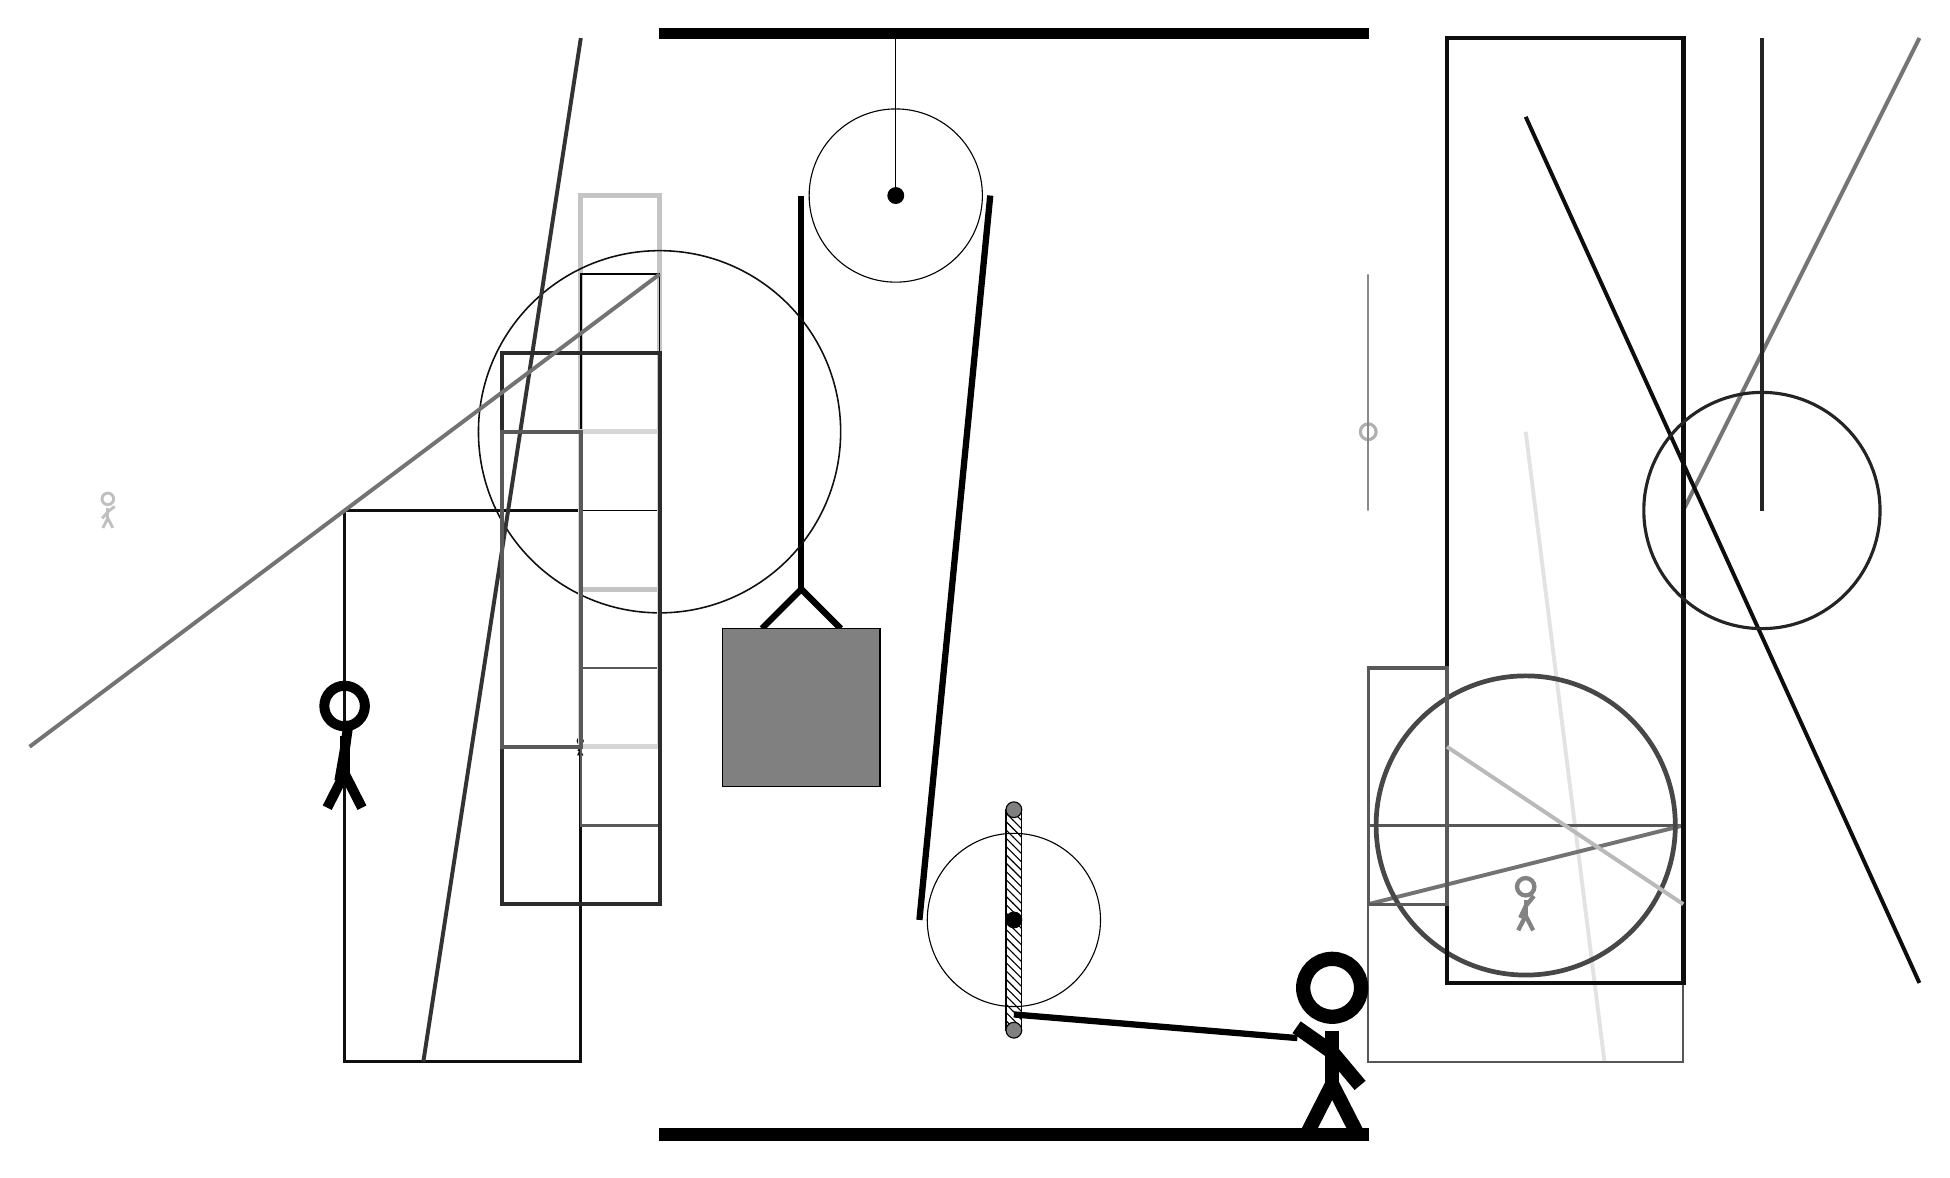
\begin{tikzpicture}
			%%%%% START %%%%%
			
			\draw[fill=black] (-2, 14) rectangle (7, 14.125);
			
			\draw (1, 12) circle (1.1);
			\draw[fill=black] (1, 12) circle (0.1);
			\draw (1, 14) -- (1, 12);
			
			\draw[fill=white](2.5, 2.8) circle (1.1);
			\draw[fill=black] (2.5, 2.8) circle (0.1);
			\draw[pattern=north west lines, pattern color=black] (2.4, 4.2) rectangle (2.6, 1.4);
			\draw[fill=black!50] (2.5, 4.2) circle (0.1);
			\draw[fill=black!50] (2.5, 1.4) circle (0.1);
			
			\draw[line width=0.8mm] (-0.7, 6.5) -- (-0.2, 7.0) -- (0.3, 6.5);
			\draw[fill=black!50] (-1.2, 6.5) rectangle (0.8, 4.5);
			
			\draw[line width=0.8mm] (-0.2, 12) -- (-0.2, 7.0);
			\centerarc[line width=0.8mm](1, 12)(0:180:1.2000000000000002);
			\draw[line width=0.8mm](2.2, 12) -- (1.3, 2.8);
			\centerarc[line width=0.8mm](2.5, 2.8)(180:270:1.2000000000000002);
			\draw[line width=0.8mm](2.5, 1.6) -- (6.1, 1.3);
			
			\draw[line width=0.6mm, color=black!23] (-3, 12) rectangle (-2, 7);
			
			\draw[line width=0.5mm, color=black!11](9, 9) -- (10, 1);
			\draw[line width=0.4mm, color=black!94] (-3, 1) rectangle (-6, 8);
			\node[line width=0.3mm, color=black!94] at (-3, 5) {\Strichmaxerl[1][61][17]};
			\draw [line width=0.2mm, color=black!94](-2, 9) circle (2.3);
			\node[line width=0.5mm, color=black!49] at (9, 3) {\Strichmaxerl[3][65][51]};
			
			\draw[line width=0.5mm, color=black!54](11, 8) -- (14, 14);
			\draw[line width=0.3mm, color=black!66] (7, 4) rectangle (11, 1);
			\draw[line width=0.5mm, color=black!55](7, 3) -- (11, 4);
			\draw[line width=0.2mm, color=black!99] (-3, 11) rectangle (-2, 8);
			\draw [line width=0.4mm, color=black!31](7, 9) circle (0.1);
			\draw [line width=0.6mm, color=black!72](9, 4) circle (1.9);
			\draw[line width=0.5mm, color=black!80](-5, 1) -- (-3, 14);
			
			\draw[line width=0.3mm, color=black!65] (-3, 4) rectangle (-2, 6);
			\draw[line width=0.6mm, color=black!16] (-2, 5) rectangle (-3, 9);
			\draw[line width=0.6mm, color=black!95] (8, 2) rectangle (11, 14);
			
			\node[line width=0.7mm, color=black!100] at (-6, 5) {\Strichmaxerl[7][80][82]};
			\draw[line width=0.5mm, color=black!83] (-2, 3) rectangle (-4, 10);
			\draw[line width=0.5mm, color=black!95](9, 13) -- (14, 2);
			
			\draw[line width=0.3mm, color=black!46] (7, 11) rectangle (7, 8);
			\draw[line width=0.5mm, color=black!86](12, 8) -- (12, 14);
			
			\draw[line width=0.4mm, color=black!65] (7, 3) rectangle (8, 6);
			\draw [line width=0.4mm, color=black!86](12, 8) circle (1.5);
			\draw[line width=0.5mm, color=black!27](11, 3) -- (8, 5);
			\draw[line width=0.5mm, color=black!55](-2, 11) -- (-10, 5);
			
			\node[line width=0.3mm, color=black!25] at (-9, 8) {\Strichmaxerl[2][50][38]};
			
			\draw[line width=0.5mm, color=black!65] (-4, 5) rectangle (-3, 9);
			\draw[line width=0.7mm, color=black!36] (9, 6) rectangle (9, 6);
			
			\node at (6.5, 1.2) {\Strichmaxerl[10][-35][-50]};
			
			\draw[fill=black] (-2, 0) rectangle (7, 0.15);
			
			%%%%% END %%%%%
		\end{tikzpicture}
	\end{figure}	
\end{document}